% !TEX encoding = UTF-8
% !TEX TS-program = pdflatex
% !TEX root = ../tesi.tex
% !TEX spellcheck = it-IT

%**************************************************************
\chapter{Conclusioni}
\label{cap:conclusioni}
%**************************************************************

\intro{Breve introduzione al capitolo}\\
Capitolo contenente le conclusioni sull'attività di Stage, dal consuntivo alle valutazioni personali.

%**************************************************************
\section{Bilancio finale}
\begin{figure}[!ht] 
    \centering 
    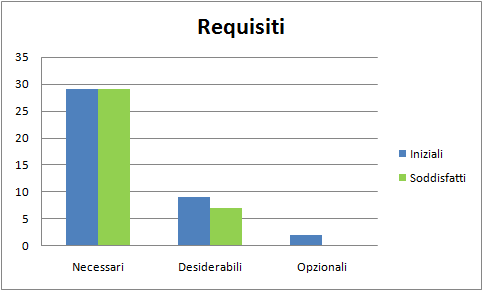
\includegraphics[width=0.9\columnwidth]{consuntivo_requisiti} 
    \caption{Grafico di rapporto tra requisiti totali e soddisfatti}
\end{figure}
Gli obiettivi per la riuscita soddisfacente dello Stage sono stati fissati subito dopo la fase iniziale di formazione. Tali obiettivi si sono concretizzati tramite l'individuazione dei requisiti dell'applicazione \emph{SkillMatrix}, ovvero le caratteristiche e le funzionalità che l'applicativo deve avere per soddisfare ed essere utile al Committente.\\
I requisiti individuati e riportati nella sezione \ref{sec:requisiti} sono serviti soprattutto per garantire che le funzionalità desiderate per \emph{SkillMatrix} siano state implementate. Nel mio caso, tali requisiti sono stati suddivisi in \textbf{necessari}, \textbf{desiderabili} ed \textbf{opzionali}. I requisiti \textbf{necessari} formalizzano le funzionalità base e imprescindibili per il corretto funzionamento dell'applicazione, ovvero i requisiti che devono essere implementati completamente. \textbf{Desiderabili} sono invece i requisiti che rappresentano le funzionalità aggiuntive che accrescono il valore del prodotto, portando un beneficio in termini di usabilità o estensione. I requisiti \textbf{opzionali}, invece, rappresentano \emph{feature} minori, ovvero che non sono ritenuti prioritari o importanti al fine della realizzazione del progetto.\\
Sulla base di ciò, al termine della mia attività di Stage ho realizzato pienamente tutti i requisiti \textbf{necessari}, che costituivano la parte predominante dei requisiti identificati, più la quasi totalità dei requisiti \textbf{desiderabili}. Per ragioni di pianificazione e confronto con il Responsabile Aziendale, abbiamo preferito dare priorità agli elementi base della gestione utente, piuttosto che alla realizzazione delle \emph{feature} aggiuntive, le quali, se necessario, saranno sviluppate in un secondo momento.\\
La piccola quantità di requisiti \textbf{opzionali} non è stata implementata, in quanto si tratta di funzionalità minori, ritenute meno importanti e quindi tralasciate.

%**************************************************************
\section{Problematiche incontrate}
L'applicazione di un modello di sviluppo \emph{Agile} è stata relativamente difficoltosa, a primo impatto. Questo modello, a mio avviso, si applica più efficacemente a sviluppatori con solida esperienza, data la sua versatilità e flessibilità di utilizzo. Infatti, se si applica la metodologia \emph{Agile} senza delle procedure adeguate, il risultato può essere imprevedibile.\\
Sebbene all'interno dell'azienda ci fossero delle procedure ben consolidate per l'applicazione di questo modello, la sua attuazione da parte mia non è stata immediata. Ciò è stato anche causato dall'assenza di esperienza da parte mia delle tecnologie aziendali per la gestione dello sviluppo software, per colmare la quale è stata impiegata la prima settimana di Stage.\\
La settimana iniziale di formazione ha contribuito ampiamente a colmare le mie lacune teoriche e pratiche sull'attuazione di una metodologia \emph{Agile} e sulla sua implementazione a livello di strumenti aziendali.\\
Ho riscontrato la stessa mancanza di conoscenze per quanto riguarda gli strumenti di automazione e di testing che ho utilizzato in questo Stage. Questo problema è stato facilmente risolvibile, in quanto la documentazione presente online dei framework che ho utilizzato è ampiamente esaustiva; inoltre la facilità di interfacciamento tra le varie componenti dello stack tecnologico che ho utilizzato, ha permesso una ancora maggiore efficienza nell'apprendimento e nell'applicazione di queste tecnologie.\\
Per ultima, forse la realtà che è stata più distante dalla mia consuetudine di studente, la metodologia \emph{Test Driven} si è rivelata tanto efficace quanto difficile da applicare. Il metodo di sviluppo che sta alla base del \emph{Test Driven Developement} è stato molto lontano da quello che ho applicato nei progetti della mia carriera universitaria.

%**************************************************************
\section{Conoscenze acquisite}
L'acquisizione delle conoscenze necessarie ad applicare la metodologia \emph{Agile} con criterio e organizzazione è stata per me un obiettivo fondamentale per la buona riuscita dello Stage e per la mia carriera futura. Sicuramente l'aggiunta dei \emph{framework} che implementano questa tecnologia che ho imparato a conoscere durante lo Stage ampliano molto il mio bagaglio culturale di sviluppatore.\\
Ritengo che la metodologia di sviluppo \emph{Agile}, se applicata con criterio, sia molto efficace e durante il corso di questo Stage ho imparato a mettere in pratica i suoi principi, grazie anche all'aiuto del mio Responsabile Aziendale Marco Albarelli.\\
Un'altra metodologia che sono stato molto soddisfatto di aver applicato è il \emph{Test Driven Developement}. Sebbene il primo impatto spinga a vedere lo sviluppo \emph{Test Driven} come molto oneroso in termine di tempo e, forse, ripetitività, a lungo andare gli effetti di un investimento iniziale sono molto positivi. Questa metodologia permette di risparmiare molto lavoro postumo e aumenta la manutenibilità del codice, garantendo la qualità del codice stesso ancora prima della sua stesura. Inoltre, quando si ha a che fare con linguaggi di programmazione molto liberi come JavaScript, l'apporto di test alla scrittura di codice è pressoché obbligatorio, se davvero si vogliono scrivere applicazioni stabili e manutenibili.\\
Ultimo ma non meno importante, ho potuto esprimere al meglio il mio interesse verso il \emph{framework} AngularJS. Questo \emph{framework}, oltre ad avere delle funzionalità molto utili per lo sviluppo di applicazioni \gls{front-end}, garantisce una compatibilità molto alta con altri strumenti utili per lo sviluppo di applicazioni \emph{client-side}, come gli strumenti di testing e automazione.\\
La scrittura di applicazioni web con AngularJS e Bootstrap risulta molto intuitiva e veloce, soprattutto se supportatat da strumenti come Grunt e Karma, che ho imparato ad utilizzare approfonditamente durante questo Stage. 

%**************************************************************
\section{Valutazione personale}
La mia valutazione personale sull'attività di Stage che ho svolto è estremamente positiva. Il confronto con una realtà lavorativa mi ha portato all'acquisizione di esperienze più profonde e concrete rispetto ad un progetto didattico.\\
Il personale di IKS è stato sempre molto disponibile a chiarire i miei dubbi, invitandomi a partecipare attivamente ed a riflettere sulle soluzioni da adottare, così da farmi crescere ulteriormente sia come sviluppatore che come persona; ringrazio davvero molto l'azienda e l'università per avermi concesso questa opportunità.\\
Infine penso che le tecnologie che ho applicato durante lo Stage mi saranno utili nel futuro prossimo, sia che le vada ad applicare direttamente, sia che vada ad adottare un diverso \emph{stack} tecnologico. In ogni caso, ho aumentato la mia sicurezza  ed efficienza nell'applicazione di queste conoscenze, e penso che ciò sia molto utile.

